\documentclass[10pt]{beamer}

%STANDARD PREAMBLE
%https://tex.stackexchange.com/questions/68821/is-it-possible-to-create-a-latex-preamble-header
\usepackage{/Users/mwojno01/Research/Learning/latex_preamble/beamer_preamble}

%
%% ALLOW FOR ITEMIZE ENVIRONMENTS WITH NO PRECEDING
% SPACING, IF DESIRED
% Reference: https://tex.stackexchange.com/questions/86054/how-to-remove-the-whitespace-before-itemize-enumerate
%\usepackage{enumitem}% http://ctan.org/pkg/enumitem 
\usepackage{paralist}

\title{Hierarchical Bayesian Linear Regression}

\begin{document}

\maketitle

\section{Motivation}
\begin{frame}{Setting}
Suppose we collect multiple measurements (covariates \& outcomes) within each of several groups.
\vfill 

\metroset{block=fill}
\begin{block}{Example}
\begin{itemize}
\item \textbf{Outcome:} math score	
\item \textbf{Covariate:} socioeconomic status (SES)	
\item \textbf{Observational units:} 10th graders
\item \textbf{Groups:} 100 public high schools 
\end{itemize}

%We want to relate math score (outcome) to socioeconomic status (SES) for 10th grade children from 100 different urban public high schools. 	

\end{block}
\end{frame}

\begin{frame}{Separate regression lines}

\scriptsize 	
What if we fit a separate regression for each school?

\begin{figure}
\begin{center}
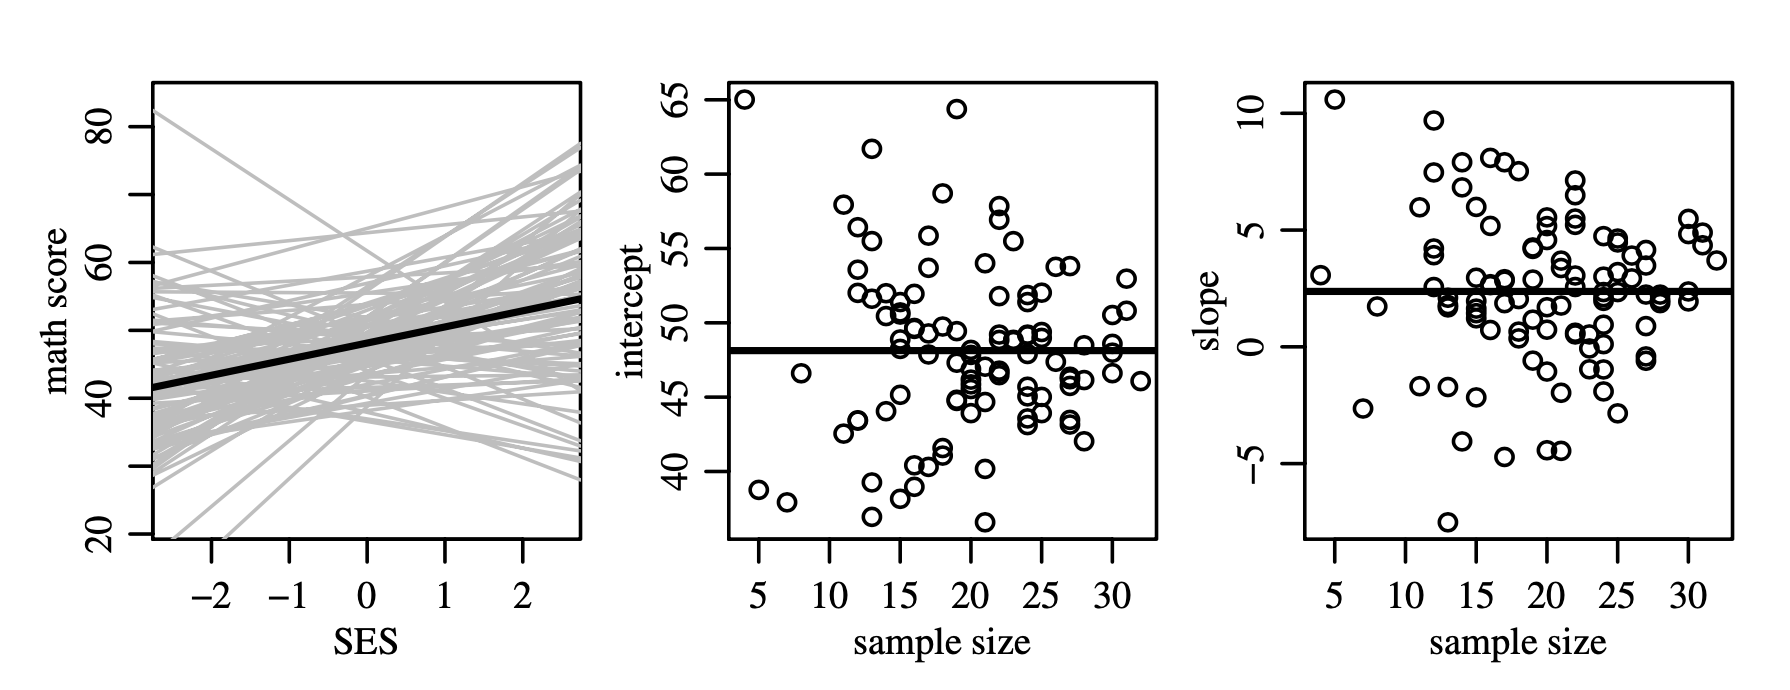
\includegraphics[width=\textwidth]{images/hoff_hierarchical_linreg}
\caption{Least squares regression lines;  estimates vs. group sample sizes} 
\end{center}
\end{figure}

\textit{Observations?} \pause Schools with ...
\begin{itemize}
\item ... the highest sample sizes tend to have regression coefficients that are close to the average.
\item ... the lowest sample sizes tend to have regression coefficients that are more extreme.
\end{itemize}

\vfill 

\bottomtext{\hfill Hoff, P. D. (2009). A first course in Bayesian statistical methods (Vol. 580). New York: Springer.}
\end{frame}


\begin{frame}{Problem and solution}

\metroset{block=fill}
\begin{block}{The problem}
Regression estimates are unstable when information is low.

{\blue{Small Datasets} }  \\
\textit{Example:} Some groups can have few observations \\

{\blue{Large Datasets} } \\
\textit{Example:} \pause  There exists a rare, but highly predictive, binary covariate. 	{\tiny (The estimation becomes especially hard if there are many other covariates, some of them also highly predictive, and some of them correlated with the rare binary covariate.)}
\end{block}
	
\metroset{block=fill}
\begin{block}{The remedy}
Stabilize the regression estimates by sharing information across groups, using a hierarchical model.
\end{block}

\end{frame}

\section{Model}
\begin{frame}{A model}
Consider a Bayesian hierarchical linear regression.   

\begin{align*}
\+\mu &\sim  \N (\+m_0,\+V_0) \\
\+\Sigma &\sim \InvWish(\eta_0, \+\Psi_0) \\
\+\beta_j &\iid \N(\+\mu,  \+\Sigma) \\
\sigma^2 &\sim \InverseGamma (\frac{\nu_0}{2}, \frac{\nu_0}{2} \sigma_0^2) \\
y_{ij}  &\indsim \N(\+\beta_j^T \+x_{ij} , \sigma^2) 
\labelit \label{eqn:hierarchical_linear_regression}
\end{align*}
	
\metroset{block=fill}
\begin{block}{The idea}
 \scriptsize We take the regression to be hierarchical in the sense that we take the regression weights $\+\beta_j$ to be distinct for each of $j=1,...,J$ groups,  but we assume that the $\+\beta_j$'s are drawn from some distribution.     The model allows for ``sharing statistical strength" in the sense that uncertainty about the $j$th group's regression parameters,  to the extent that it exists,  can be reduced by borrowing information from the other groups $k \neq j$.    In other words,  for grouped data,  we allow the information from the other groups to play the role that is played by the prior in Bayesian linear regression. (\textit{Explain.})
\end{block}
\end{frame}

\section{Inference}

\begin{frame}{Inference on ``Population-level" (i.e. across-group) quantities}
\alert{Key Insight}: The top part of the model behaves like a Bayesian multivariate normal model,    but where the ``data" are the (latent) regression weights,  $\+\beta_1, ...,\+\beta_J$. 

\begin{align*}
\+\mu \cond  \+\beta_1, ...,\+\beta_J,  \+\Sigma &\sim \N(\+m^\prime,  \+V^\prime) \\
\+m^\prime &= \+V^\prime \bigg( \+V_0^{-1} \+m_0 + \greenmathbox{J} \+\Sigma^{-1} \bluemathbox{\overline{\+\beta}} \bigg),  \quad \quad \overline{\+\beta} := \frac{1}{J} \sum_{j=1}^J \+\beta_j \\ 
\+V^\prime &=  \bigg( \+V_0^{-1} + \greenmathbox{J} \+\Sigma^{-1} \bigg)^{-1} \\
& \\ 
\+\Sigma \cond \+\beta_1, ...,\+\beta_J,  \+\mu &\sim \InverseWishart (\eta^\prime, \+\Psi^\prime) \\
\eta^\prime &= \eta_0 + \greenmathbox{J} \\
\+\Psi^\prime &= \+\Psi_0 + \greenmathbox{\ds\sum_{j=1}^J} (\redmathbox{\+\beta_j} - \+\mu) (\redmathbox{\+\beta_j} -\+\mu)^T \\
\labelit \label{eqn:hierarchical_linear_regression_ccs}
\end{align*}


\end{frame}

\begin{frame}{Recall: Multivariate normal updates (for comparison)}

\begin{align*}
\+\mu  \cond \+\Sigma, \+x &\sim \N_{d}(\+m',\+V' )  \labelit\label{eqn:normal_model_complete_conditional_on_mu} \\
\+m'  &=  \+V'  \bp{\+V_0^{-1} \+m_0 + \greenmathbox{N} \+\Sigma^{-1}  \bluemathbox{\bar{\+x}} } \\
\+V' &= \bp{\+V_0^{-1} +  \greenmathbox{N} \+\Sigma^{-1} }^{-1} \\
\intertext{and}
\+\Sigma \cond \+\mu,  \+x  &\sim \InverseWishart(\nu',  \+\Psi')  \\
\nu' &=  \nu_0 + \greenmathbox{N} \\
\+\Psi' &= \Psi_0 + \greenmathbox{\ds\sum_{i=1}^N}  (\redmathbox{\+x_i} - \+\mu) (\redmathbox{\+x_i} - \+\mu)^T  
\end{align*}
	
\end{frame}

\begin{frame}{Inference on group-specific regression weights}
\alert{Key Insight}: This part of the model behaves like a Bayesian linear regression model,    but where the ``prior" mean and variance becomes the ``empirical" mean and variance of the (latent) regression weights,  $\+\beta_1, ...,\+\beta_J$ across groups. 

\begin{align*}
\+\beta_j \cond \+\Sigma,  \+\mu, \sigma^2,  \+y & \sim  \N(\+\mu_j^\prime,  \+\Sigma_j^\prime) \\
\+\Sigma_j^\prime &= \bigg( \explaintermbrace{between-group precision}{\+\Sigma^{-1}} + \explaintermbrace{within-group precision}{\frac{1}{\sigma^2} \+X_j^T \+X_j} \bigg)^{-1} \\
\+\mu_j^\prime &= \+\Sigma_j^\prime \bigg( \explaintermbrace{\tiny between-group precision-weighted mean}{\+\Sigma^{-1} \+\mu} + \explaintermbrace{\tiny within-group precision-weighted mean}{\frac{1}{\sigma^2} \+X_j^T \+y_j} \bigg) 
\end{align*}	
\end{frame}

\begin{frame}{Recall: Bayesian linear regression (for comparison)}

In standard BLR, the updates on the regression weights are given by

\begin{align*}
\+\beta \cond \+y,  \sigma^2 & \sim \N(\+\mu,  \+\Sigma )
\intertext{where}
\+\Sigma &= \bp{ \explaintermbrace{prior precision}{\+\Sigma_0^{-1}} +  \explaintermbrace{data precision}{\frac{1}{\sigma^2} \+X^T \+X} }^{-1}  \\
\+\mu &= \+\Sigma \bp{   \explaintermbrace{\tiny prior precision-weighted mean}{\+\Sigma_0^{-1} \+\mu_0} +  \explaintermbrace{\tiny data precision-weighted mean}{\frac{1}{\sigma^2} \+X^T  \+y}}  \\
\labelit \label{eqn:posterior_bayesian_lin_regression_with_known_obs_var}
\end{align*}

	
\end{frame}



\begin{frame}{Inference on observation noise}

\alert{Key Insight}: We estimate the observation noise by simply pooling the residuals across all the groups. 

\begin{align*}
\sigma^2 \cond \+\beta_1, ...,\+\beta_J,  \+y & \sim \InverseGamma
\bigg( \half (\nu_0 + N),  \half (\nu_0 \sigma_0^2 + \text{SSR}(\+\beta)\bigg)\\ 
N &:= \sum_{j=1}^J n_j \\
\text{SSR(\+\beta)} &:= \ds\sum_{j=1}^J \ds\sum_{i=1}^{n_j}  (y_{ij} - \+\beta_j^T \+x_{ij})^2 \\
\end{align*}	
\end{frame}

\begin{frame}{Results}
The hierarchical model is able to share information across groups. 
\begin{columns}
\begin{column}{.45\textwidth}
Posterior expectations of the 100 school-specific regression lines, with the average line given in black.	
\end{column}
\begin{column}{.45\textwidth}
\begin{center}
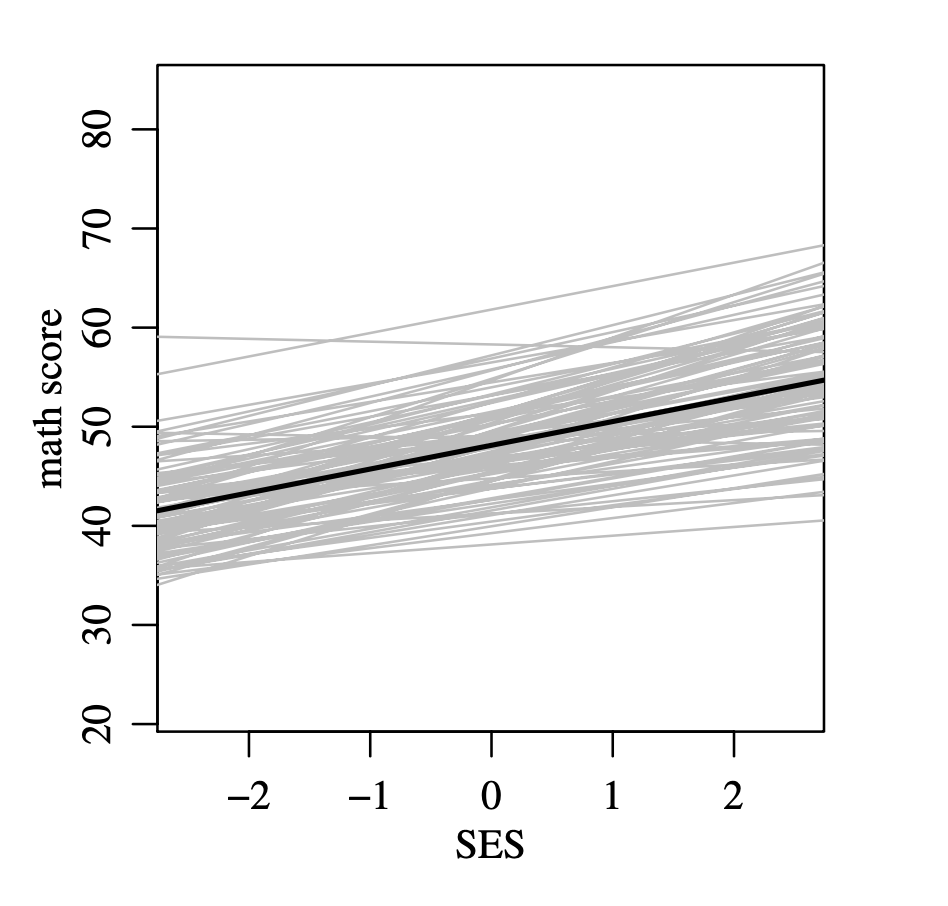
\includegraphics[width=\textwidth]{images/hoff_smoothed_linreg_lines} 
\end{center}
\end{column}
\end{columns}


\textit{Observations?} \pause
\begin{itemize}
\item Extreme regression lines are shrunk towards the across-group average. {\tiny (In particular, hardly any of the slopes are negative after sharing information.)}
\item Schools with less information have greater shrinkage.
\end{itemize}
\end{frame}

\end{document}